% Pacotes
\documentclass[12pt]{article}
\usepackage{adjustbox}
\usepackage[utf8]{inputenc}
\usepackage{amsmath}
\usepackage{hyperref}
\usepackage{sbc-template}
\usepackage{fancyvrb}
\usepackage{amsfonts}
\usepackage{amsmath}
\usepackage{graphicx,url}

\sloppy

\title{Memória Virtual e Algoritmos de Paginação}

\author{Ricardo Henrique Brunetto (94182)\\
				Rafael Rodrigues dos Santos (94075)\\
				Thais Aparecida Silva Camacho (93807)}

\address{Departamento de Informática -- Universidade Estadual de Maringá (UEM)\\
	Maringá -- PR -- Brasil
}

\begin{document}

\maketitle

{\resumo{Este artigo visa a apresentar um resumo dos principais algoritmos de paginação implementados por Sistemas Operacionais Modernos, analisando sua vantagens e desvantagens.}}

\section{Introdução}

A princípio, fazer-se-á um apanhado geral a respeito de conceitos básicos que fundamentam o uso dos Algoritmos de Paginação. É importante que se faça claro o escopo deste artigo, não aprofundando o contexto que os algoritmos de paginação estão inseridos, mas suficientemente orientando o entendimento de sua funcionalidade e a motivação para existência.

\subsection{Memória Virtual}\label{sec:memvir}

Memória virtual é uma técnica que possibilita que programas muito maiores que a memória disponível possam ser executados, sendo desnecessário uma arquitetura específica para cada aplicação. Nesse sentindo, a memória virtual funciona como um espaço variável é reservado no disco rígido que passa a executar os programas quando o sistema operacional percebe que a memória RAM não tem mais espaço suficiente. A ideia básica é que cada programa tenha seu próprio espaço de endereçamento divididos em blocos chamados \textbf{páginas}.

A memória virtual foi criada para resolver um problema antigo e que assombrava à computação há anos: o tamanho dos softwares estava ficando cada vez maior, mas as memórias não acompanhavam esse crescimento na mesma proporção.
Antes da criação da memória virtual, uma solução foi adotada, a de sobreposição (\textit{overlays}), a qual permitia que varias memórias fossem executadas ao mesmo tempo. No entanto, essa solução ainda tinha um empecilho, a divisão do programa em módulos deveria ser feita manualmente pelo programador o que atrasava o processo todo. Dessa forma, a memória virtual permitiu que todo processo fosse realizado virtualmente pelo sistema operacional, facilitando a vida do programador e permitindo que programas maiores que a memória principal possam ser executados.

A grosso modo, a Memória Virtual pode ser vista como uma generalização da ideia do registrador-limite e do registrador-base. Assim, é possível que toda a memória física seja mapeada em unidades menores. Isso significa que a Memória Virtual funciona bem para sistemas que suportam multiprogramação, permitindo mais de um processo em execução

\subsection{Paginação}

Dessa forma, é necessário aplicar uma técnica para gerenciar as partes do programa (páginas) que serão carregados para a Memória Principal. Essa técnica é chamada de \textbf{Paginação}. Cada página é uma série contígua de endereços, sendo mapeadas na memória física. Isso significa que, embora tais páginas sejam mapeadas para a memória principal, nem todas precisam estar simultaneamente na memória principal.

Conforme a estrutura da Memória Virtual, explanada superficialmente na Seção \ref{sec:memvir}, os endereços podem ser gerados através da indexação dos registradores de base, de segmento ou através de outras técnicas que envolvam como entrada o endereço real. Esses endereços são denominados \textbf{endereços virtuais} e integram o \textbf{espaço de endereçamento virtual}. Esta conversão deve ser projetada de modo que, caso não haja memória virtual no sistema computacional, o espaço de endereçamento real e virtual.

Dessa forma, as Páginas são fragmentos do espaço de endereçamento virtual, ao passo que as Molduras de Páginas (\textit{page frames}) são as correspondentes na memória física, tendo ambas o mesmo tamanho.

Ao utilizar Memória Virtual, o endereço virtual não é inserido diretamente no barramento, mas sim previamente processado pela Unidade de Gerenciamento de Memória (MMU - \textit{Memory Management Unit}), responsável por mapear endereços virtuais em endereços físicos. A memória em si desconhece a existência do MMU e interpreta unicamente as requisições de leitura e escrita vindas do barramento. Portanto, deve-se ter compatibilidade entre o endereço virtual e o endereço real.

Por fim, quando determinado endereço de uma página é requisitado e se encontra na memória, então é utilizado. Caso contrário, ocorre uma interrupção de falta de página e o sistema operacional trata a requisição buscando a página desejada e carregando-a em memória. Nesses casos, o espaço de endereçamento do programa já estará lotado e, então, deve-se adotar uma política que permita realizar a \textbf{substituição de páginas} (vide Seção \ref{sec:algpag} para mais detalhes).

\section{Algoritmos de Substituição de Páginas}\label{sec:algpag}

Quando ocorre uma falta de página (\textit{page fault}), o sistema operacional precisa escolher uma página a ser removida da memória para liberar espaço a fim de trazer uma nova página para a memória. Se a página a ser removida, tiver sido modificada enquanto esteve na memória, tal página deverá ser reescrita no disco. No entanto, se a página não tiver sido modificada, não é necessário reescrevê-la, pois a cópia em disco já estará atualizada.

A página que está sendo trazida para a memória simplesmente sobrepõe a página que está sendo removida. Existem vários algoritmos que realizam a escolha da página a ser sobreposta. Tais algoritmos são apresentados a seguir.

\subsection{Algoritmo Ótimo}

O algoritmo ótimo é o que apresenta o melhor desempenho computacional e o que minimiza o número de faltas de páginas. No entanto, sua implementação é praticamente impossível.

A idéia do algoritmo é retirar da memória a página que vai demorar mais tempo para ser referenciada novamente. Para isso, o algoritmo precisaria saber, antecipadamente, todos os acessos à memória realizados pela aplicação, o que é impossível em um caso real. Isso porque há dinamismo durante a execução de processo e o acesso à memória (bem como o uso de outros recursos) pode estar condicionado a fatores não previsíveis (entradas do usuário, respostas de requisições, etc).

Por estes motivos, o algoritmo ótimo só é utilizado em simulações para se estabelecer o valor ótimo e analisar a eficiência de outras propostas elaboradas.

\subsection{Algoritmo NUR (Não usada recentemente)}

O algoritmo de substituição de página \textit{NRU} utiliza os dois bits de status, o bit referenciada (\textbf{R}) e o bit modificada (\textbf{M}), associados a cada página virtual referenciada pela MMU, como mostra a figura \ref{ram-nru-1}. 

\begin{figure}
	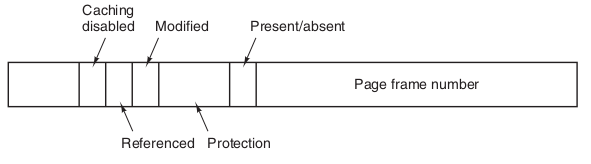
\includegraphics[scale=0.6]{ram-nru-1.png}
    \centering
    \caption{Bits R (Referenced) e M (Modified) na entrada de uma tabela de páginas}
    \label{ram-nru-1}
\end{figure}

Tais bits servem para o sistema operacional coletar estatísticas de páginas de uso, pois com eles o sistema operacional consegue saber quais páginas estão sendo usadas e quais não estão. Com isso, tem-se que 

\begin{itemize}
\renewcommand{\labelitemi}{}
\item bit R (referenciada): é 1 se a página foi lida ou escrita;
\item bit M (modificada): é 1 se a página foi escrita.
\end{itemize}

Dessa forma, quando um processo se inicia, os dois bits em questão, são colocados em 0, para todas as suas páginas. Periodicamente, o bit R é limpo de modo que diferencie as páginas que não foram referenciadas recentemente daquelas que foram. O bit M não é limpo, pois o sistema operacional precisa saber se deve escrever a página no disco.

Quando ocorre uma falta de página, o sistema operacional inspeciona todas as páginas, separando-as nas seguintes categorias

\begin{itemize}
\renewcommand{\labelitemi}{}
\item Classe 0 (00): não referenciada, não modificada.
\item Classe 1 (01): não referenciada, modificada.
\item Classe 2 (10): referenciada, não modificada.
\item Classe 3 (11): referenciada, modificada.
\end{itemize}

Dessa forma, o algoritmo NUR remove de maneira aleatória uma página da classe de ordem mais baixa.

\section{Algoritmo FIFO}

O FIFO (\textit{First-in, First-out} - primeira a entrar, primeira a sair) é um algoritmo de substituição de páginas de baixo custo e de fácil implementação que consiste em substituir a página que foi carregada há mais tempo na memória (a primeira página a entrar é a primeira a sair).

Escolher a página que está há mais tempo na memória pode não ser uma opção eficiente. Isso porque um determinado processo pode executar um trecho do código em \textit{loop}, repetindo-o em determinada quantidade de tempo, ou ainda, necessitar de um trecho específico em todas as partes de seu processamento, necessitando de uma página que fora previamente carregada.

Isso significa que esta escolha não leva em consideração se a página está sendo muito utilizada ou não, o que não é muito adequado pois pode prejudicar o desempenho do sistema. Por este motivo, o FIFO apresenta uma deficiência denominada \textbf{anomalia de Belady}: a quantidade de falta de páginas pode aumentar quando o tamanho da memória também aumenta, pois as páginas mais frequentemente usadas podem ser retiradas assim como as pouco frequentemente usadas.

Por estas razões, o algoritmo FIFO puro é muito pouco utilizado. Contudo, sua principal vantagem é a facilidade de implementação: uma lista de páginas ordenada pela “idade”. Dessa forma, na ocorrência de uma falta de página a primeira página da lista será substituída e a nova será acrescentada ao final da lista. Por outro lado, 

\section{Algoritmo da Segunda Chance}

O algoritmo de substituição de página da \textit{Segunda Chance} é uma tentativa de melhoramento do algoritmo anterior. Dessa forma, tal algoritmo possui o funcionamento do algoritmo FIFO, com o acréscimo do bit referenciada (R). Com isso, evita-se o problema de se jogar fora uma página intensamente usada, simplesmente inspecionando o bit R da página mais antiga, ou seja, da primeira página da fila. Caso o bit R seja 0, essa página além de ser mais antiga, não estará sendo usada, de modo que será substituída imediatamente. Caso contrário, bit R seja 1, ele será colocado para 0 e a página será enviada para o final da fila de páginas. 

Um exemplo é representado na figura \ref{ram-second-chance-1}. Supondo que no instante 20 tenha ocorrido uma falta de página. A página mais antiga é a página A, que chegou no instante 0 quando o processo foi iniciado. Se o bit R da página A for 0, então ela é retirada da memória, tendo sua cópia em disco atualizada se houver sido modificada, ou caso não tenha sido modificada, será simplesmente abandonada. Todavia, se o bit R for 1, a página A será colocada no final da fila e o seu tempo será atualizado para 20. O bit R é colocado em 0, e a busca por uma página a ser substituída continua a partir da página B, como é representado na figura \ref{ram-second-chance-1}.

\begin{figure}
	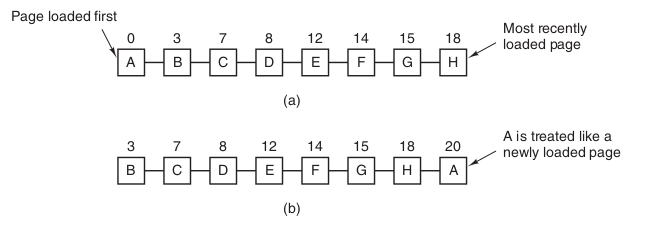
\includegraphics[scale=0.6]{ram-second-chance-1.png}
    \centering
    \caption{Representação do funcionamento do Algoritmo da Segunda Chance}
    \label{ram-second-chance-1}
\end{figure}

\subsection{Algoritmo do Relógio}

O algoritmo de substituição de página do \textit{Relógio} visa um melhoramento do algoritmo anterior. A única mudança é no formato da lista que passa a ter um formato circular (parecido com um relógio), como mostra a figura \ref{ram-clock-1}. Um ponteiro aponta para a página mais antiga, ou seja, para a `cabeça' da lista.

Quando ocorre uma falta de página, a página mais antiga, apontada pelo ponteiro, será verificada. Caso o bit R dessa página seja 0, tal página será substituída, a nova página será inserida em seu lugar e o ponteiro avançará, uma posição. Tal processo é repetido até uma página antiga com bit $R = 0$ seja encontrada e retirada.

\begin{figure}
	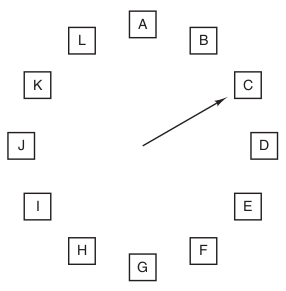
\includegraphics[scale=0.6]{ram-clock-1.png}
    \centering
    \caption{Representação do Algoritmo do Relógio}
    \label{ram-clock-1}
\end{figure}

\subsection{Algoritmo MRU (Menos recentemente usada)}

O algoritmo de substituição de página \textit{MRU} parte do princípio que as páginas usadas com mais frequência nas ultimas execuções provavelmente serão muito utilizadas novamente. Desse modo, quando houver uma falta de página o algoritmo elimina a página não utilizada pelo período de tempo mais longo.

A implementação do algoritmo MRU demanda alto custo. Para implementá-lo é necessário manter uma lista encadeada de todas as páginas na memória. Onde a página mais recentemente usada se encontra no início da lista e a página menos recentemente usada se encontra no final. Dessa forma, é necessita que a lista seja atualizada para cada execução, além do que, uma página será buscada, se encontrada ela será excluída e posicionada
na frente da lista.

Contudo, o algoritmo é possível de ser implementado tanto em hardware como em software. Ambas as implementações são apresentada a seguir.

\subsubsection{MRU em hardware}

O MRU em hardware necessita de um contador de 64 bits, que é incrementado automaticamente após a execução de cada instrução. Além disso, cada entrada da tabela de páginas deve ter um campo extra para armazenar o valor do contador. Após cada referência à memória, o valor atual do contador é armazenado nesse campo adicional da entrada da tabela de páginas correspondente à página que acabou de ser referenciada. Ao ocorrer uma falta de página, o sistema operacional examina todos os campos contadores da tabela de páginas a fim de encontrar o menor deles. Dessa forma, a página correspondente a esse menor valor será a `menos recentemente usada'.

O problema dessa implementação, é que poucas máquinas possuem esse hardware, dessa forma tal implementação acaba não sendo utilizada pelos projetistas de sistemas operacionais.

\subsubsection{MRU em Software (NFU)}

O algoritmo \textit{NFU}, algoritmo de substituição de páginas não usada frequentemente, exige para cada página um contador implementado em software. Inicialmente, o contador de cada página é zerado. A cada interrupção do relógio, o sistema operacional percorre todas as páginas na memória. Onde para cada página, o bit referenciada R, que pode estar em 0 ou 1, é adicionado ao contador correspondente. Dessa forma, consegue-se saber quantas vezes cada página foi referenciada. Na ocorrência de uma falta de página, a página que será substituída é a com menor contagem.

O problema do algoritmo NFU é que ele nunca se esquece de nada, dessa forma páginas frequentemente muito acessadas no inicio não serão candidatas para serem substituídas, mesmo que deixadas de ser acessadas no futuro.

\subsection{Algoritmo do Conjunto de Trabalho}

O algoritmo de substituição de páginas do \textit{Conjunto de Trabalho} foi concebido para reduzir substancialmente a frequência de faltas de páginas. O conjunto de trabalho pode ser definido como o conjunto de páginas que o processo referenciou durante os últimos $\tau$ segundos do tempo de execução.

O algoritmo deve determinar o conjunto de trabalho de cada processo e tê-lo na memória antes de rodar o processo, pois se todo o conjunto de trabalho estiver presente na memória, o processo será executado com poucas faltas de página até mudar para outra fase de execução. Carregar essas páginas antes de rodar novamente o processo é conhecido como \textbf{pré-paginação}.

A ideia central do algoritmo é encontrar uma página que não esteja presente no conjunto de trabalho e removê-la da memória. A figura \ref{ram-ws-1} mostra parte da tabela de páginas de uma máquina. Cada entrada contém no mínimo dois campos: o instante aproximado em que a página foi referenciada pela última vez e o bit R (referenciada).

\begin{figure}
	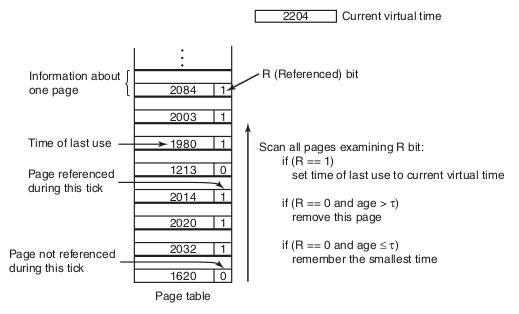
\includegraphics[scale=0.6]{ram-ws-1.png}
    \centering
    \caption{Algoritmo do Conjunto de Trabalho}
    \label{ram-ws-1}
\end{figure}

O algoritmo funciona da seguinte maneira: suponha que o hardware inicialize os bits R e M. Suponha também que cada interrupção de relógio seja ativado um software para zerar o bit R. A cada falta de página, a tabela de páginas é varrida à procura de uma página adequada para ser removido da memória.

O bit R de cada entrada da tabela de páginas é examinado. Caso o bit R for 1, o tempo virtual atual é copiado no campo \textit{Instante da última referência} na tabela de páginas, indicando que a página estava em uso no momento que ocorreu a falta de página. Como a página foi referenciada durante a interrupção de relógio atual, ela está certamente presente no conjunto de trabalho e não é uma candidata a ser removida da memória (supõe-se que o intervalor $\tau$ corresponda a várias interrupções de relógio).

Caso $R = 0$, a página não foi referenciada durante a interrupção de relógio atual e pode ser candidata à remoção da memória. Para saber se tal página deve ou não ser removida da memória, sua idade é computada e comparada com intervalo $\tau$. Onde a idade seria
tempo atual virtual menos \textit{instante da última referência} a página. Se a idade for maior que o intervalo $\tau$, faz muito tempo que tal página está ausente do conjunto de trabalho. Ela então é substituída pela nova página. Todavia, tem continuidade a atualização das entradas restantes.

Contudo, se $R = 0$ mas a idade é menor ou igual ao  intervalo $\tau$, significa que a página ainda pertence ao conjunto de trabalho. Com isso, a página é temporariamente poupada. Porém, a página com a maior idade (\textit{menor instante da última referência}) é marcada. Se a tabela toda é varrida e não se encontra nenhuma candidata a remoção, então todas as páginas estão no conjunto de trabalho. Nesse caso, se uma ou mais páginas com $R = 0$ são encontradas, a marcada com maior idade é substituída. No pior caso, todas as páginas foram referenciadas durante a interrupção de relógio atual (todas com $R = 1$). Neste caso, uma delas será escolhida aleatoriamente para remoção, preferivelmente uma página não modificada, caso exista.

\subsection{Algoritmo WSClock}

O algoritmo de substituição de páginas \textit{WSClock} é amplamente utilizado, devido à sua simplicidade. Seu funcionamento seria uma combinação do algoritmo anterior, com o algoritmo do relógio.

\begin{figure}
	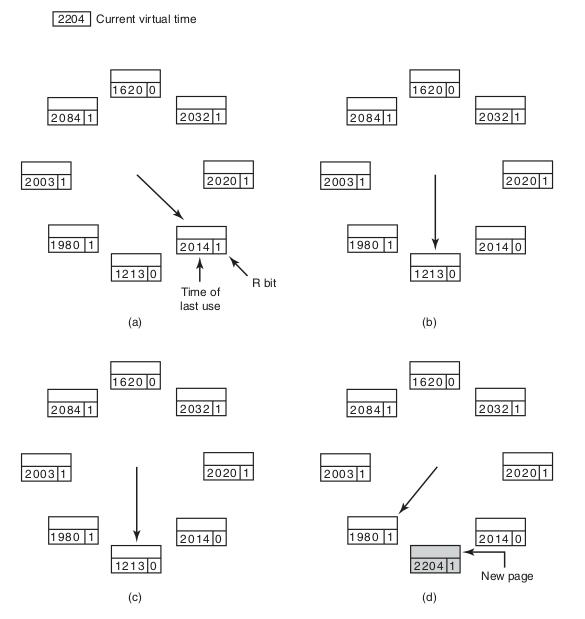
\includegraphics[scale=0.6]{ram-wsclock-1.png}
    \centering
    \caption{Representação do funcionamento do Algoritmo do Relógio}
    \label{ram-wsclock-1}
\end{figure}

A estrutura de dados utilizada é uma lista circular de molduras de página (igual no algoritmo do relógio), como mostra na figura \ref{ram-wsclock-1}(a). Inicialmente, a lista em questão é vazia. Quando a primeira página é carregada, ela é inserida na lista. À medida que mais páginas são carregadas na memória, elas são também inseridas na lista para formar um anel. Uma entrada na lista possui os campos: \textit{Instante da última referência}, \textit{bit R} e \textit{bit M} (não representado na figura \ref{ram-wsclock-1}). 

A cada falha de página, a página da cabeça é examinada primeiro. Se $R$ = 1, a página foi usada durante o ciclo de clock corrente (não é candidata à remoção). O bit R é colocado para zero e avança a cabeça à próxima página, repetindo o algoritmo para essa página. O estado posterior a essa sequência de eventos é mostrada na figura \ref{ram-wsclock-1}(b).

Todavia, quando $R = 0$ está representado na figura \ref{ram-wsclock-1}(c). Se sua idade for maior do que o intervalo $\tau$ e se essa página não estiver modificada, então ela não faz parte do conjunto de trabalho e haverá uma cópia valida em disco. A moldura de página é simplesmente removida e a nova página é inserida, como mostrado na figura \ref{ram-wsclock-1}(d). Por outro lado, se a página estiver modificada não poderá ser removida imediatamente, já que não há uma cópia válida no disco. Então o ponteiro é avançado e o algoritmo continua, pois pode haver uma página que também não pertença ao conjunto de trabalho e que não foi modificada, dando preferência a ela.

\subsubsection{Resumo dos Algoritmos}

O algoritmo ótimo substitui a última página referenciada, de todas as páginas atuais. Como é impossível determinar qual página será a última, tal algoritmo não pode ser utilizado na prática. Servindo apenas como medida-padrão de desempenho.

O algoritmo NUR divide as páginas em quatro classes, de acordo com o estado dos bits R e M. E a página escolhida é qualquer página pertencente a classe de ordem mais baixa. Tal algoritmo é fácil de implementar, mas existem outros melhores.

O algoritmo FIFO mantém as páginas em uma lista encadeada na ordem que as páginas são carregadas na memória. A remoção da página mais velha torna-se assim trivial, mas essa página pode estar ainda em uso, de forma que o FIFO não é a melhor escolha dentro todos os algoritmos.

O algoritmo da segunda chance, melhoramento do FIFO, verifica se a página está em uso antes de removê-la, analisando o estado do bit R. Caso positivo, a página é poupada. O algoritmo do relógio possui as mesmas propriedades de desempenho que algoritmo da segunda chance, porém gasta um pouco menos de tempo para executar o algoritmo.

O MRU é um excelente algoritmo, porém depende de um hardware especial. Se o hardware não está disponível, ele não pode ser utilizado. O NFU é uma tentativa, não muto boa, de simular o MRU em software.

O algoritmo do conjunto de trabalho possue um bom desempenho, mas a implementação é cara. Já o WSClock é uma variante que não somente provê um bom desempenho, como é eficiente em sua implementação.

Entre todos os algoritmos, o melhor é o WSClock, baseado no conjunto de trabalho. Ele oferece bom desempenho de paginação e pode ser implementado de forma eficiente.

\bibliographystyle{sbc}
\bibliography{References}

\end{document}
